\section{Постановка задачи} \label{p21}
\paragraph{}
Рассмотрим математическую модель двухзвенного манипулятора. Манипулятор состоит из неподвижного основания и двух абсолютно жестких звеньев $G_1, G_2$. Элементы конструкции соединены между собой двумя идеальными цилиндрическими шарнирами $O_1,$ и $O_2$ таким образом, что оба звена могут совершать движения только в горизонтальной или вертикальной плоскости. Центр масс $C_1$ звена $G_1$ лежит на луче $O_1 O_2.$ Положение центра масс $C_2$ звена $G_2$ не совпадает с положением шарнира $O_2$.

 \begin{figure}[h]
 	\centering
 	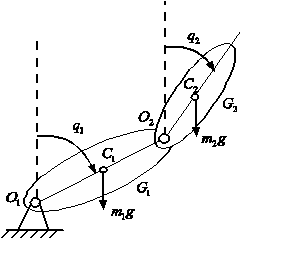
\includegraphics{manipulator}
 	\caption{Модель двузвенного манипулятора}
 	\label{fig:manip1}
 \end{figure}

Введем обозначения: $q_i (i=1, 2)$ --- углы поворотов звеньев манипулятора, показанные на рисунке; $l_i$ --- длина отрезка $O_i C_i;$ $l$ --- длина отрезка $O_1 O_2;$ $m_i$  ---  масса   $i$-го звена;   $I_i$ --- момент инерции  $i$-го звена относительно оси шарнира $O_i;$ $g$ --- ускорение свободного падения.

Выражение для кинетической энергии манипулятора имеет в таком случае следующий вид:
\begin{equation}
T = \frac12 ((I_1 + I_2 + m_2 l^2 + 2 m_2 l l_2 \cos q_2) \dot q_1^2 + (I_2 + m_2 l l_2 \cos q_2) \dot q_1 \dot q_2 + I_2 \dot q_2^2)
\end{equation}

Составим уравнения Лагранжа второго рода:

\begin{equation}
\begin{cases}
\displaystyle \frac{d}{dt} (\frac{\partial T}{\partial \dot q_1}) - \frac{\partial T}{\partial q_1} = M_1 + U_1, \\
\displaystyle \frac{d}{dt} (\frac{\partial T}{\partial \dot q_2}) - \frac{\partial T}{\partial q_2} = M_2 + U_2,
\end{cases}
\end{equation}

где $M_i$ --- момент, создаваемый силой тяжести в $i$-м шарнире. В случае манипулятора, совершающего движения в вертикальной плоскости, 
$$
\begin{array}{l}
M_1 = (m_1 l_1 + m_2 l) g \cos q_1, \\
M_2 = m_2 l_2 g \cos (q_1 + q_2),
\end{array}
$$
$U_i$ --- управление.

Из выражения для кинетической энергии $T$ находим уравнения движения

\begin{equation}
\begin{array}{l}
a_{11} \ddot q_1 + a_{12} \ddot q_2 - 2 m_2 l_1 l_2 \sin q_2 \dot q_1 \dot q_2 - m_2 l_1 l_2 \sin q_2 \dot q_2^2 = M_1 + U_1,\\ 
a_{12} \ddot q_1 + a_{22} \ddot q_2 + m_2 l_1 l_2 \sin q_2 \dot q_1^2 = M_2 + U_2,\\
a_{11} = m_2 l_1^2 + I_1 + I_2 + 2 m_2 l_1 l_{g_2} \cos q_2,\\
a_{12} = I_2 + m_2 l_1 l_{g_2} \cos q_2, a_{22} = I_2
\end{array}
\end{equation}

Пусть $q=q(q_1, q_2)^{'}$ --– вектор обобщенных координат рассматриваемой механической системы и 
$$X = \{(q^0(t), \dot q^0(t)) : [t_0, + \infty) \to R^4, \|q^0(t)\| \le g_0, \|\dot q^0(t) \| \le g_1, \|\ddot q^0(t)\| \le g_2 \}$$

есть заданное множество программных движений манипулятора в виде ограниченных дважды непрерывно дифференцируемых функций $q=q^0(t)$ с ограниченными производными при $t \in [t_0, + \infty).$ Символом $\| \cdot \|$   обозначена евклидова норма вектора.

Пусть $(q^0(t), \dot q^0(t)) \in X$ --- какое-либо программное движение, реализуемое программным управлением $U = U^0(t).$ Таким образом, для обеспечения такого движения имеет место следующее управление
$$
\begin{array}{l}
U_1^0 (t) = m_2 l_1^2 + I_1 I_2 + 2 m_2 l l_2 \cos q_2 \ddot q_1^0 (t)\\
U_2^0 (t) = I_2 \ddot q_2^0 (t) + m_2 l l_2 \cos (q_2^0 (t) - q_1^0 (t)) \dot q_1^0 (t) + m_2 l l_2 \sin(q_2^0 (t) - q_1^0 (t)) (\dot q_1^0 (t))^2 -\\
- M_2^0(t)
\end{array}
$$
где $M_1^0(t) = M_2^0(t) = 0$ для случая манипулятора в горизонтальной плоскости.

Введем возмущения $x_k = q_k - q_k^0(t), \quad \dot x_k = \dot q_k - \dot q_k^0(t), \quad k = 1, 2$

Составим уравнения возмущенного движения в векторно-матричном виде:
\begin{equation}
A^{(1)}(t, x) \ddot x = {\dot x^{'} C^{(1)}(t, x) \dot x} + Q^{(1)}(t,x) + Q^{(2)}(t, x, \dot x) + U^{(1)}, \label{2.2'}
\end{equation}

$$A^{(1)}(t, x) =
\begin{pmatrix}
I_1 + m_2 l_1^2 && m_2 l_1 l_{g_2} \cos(q_2^0(t)) + x_2 \\
m_2 l_1 l_{g_2} \cos(q_2^0(t)) + x_2  && I_2 \\
\end{pmatrix}$$

$$ C^{(1)}(t,x), \quad Q^{(1)}(t,x)=F(t,x)p(x), \quad Q^{(2)}(t,x,\dot x)=D(t,x)\dot x, $$

$$ C^{(1)}(t, x) =
\begin{mpmatrix}
- m_2 l l_2 \sin(q_2^0(t) - q_1^0(t) + x_2 - x_1) && 0 \\
0 && m_2 l l_2 \sin(q_2^0(t) - q_1^0(t) + x_2 - x_1) \\
\end{mpmatrix}, $$

$$F(t, x) =
\begin{pmatrix}
f_{11}(t,x) && f_{12}(t,x) \\
f_{21}(t,x) && f_{22}(t,x)\\
\end{pmatrix},$$

$$p(x) =
\begin{pmatrix}
\sin(x_1/2) \\
\sin(x_2/2)\\
\end{pmatrix},$$

$$D(t, x) =
\begin{pmatrix}
0 && c_{22(1)}^{(1)}(t,x) \dot q_2^0(t) \\
c_{11(1)}^{(1)}(t,x) \dot q_1^0(t) && 0 \\
\end{pmatrix},$$

$f_{11}(t,x) = 2m_2l_1l_{g_2} \cos(x_2/2) (\ddot q_2^0(t) \sin(- q_2^0(t) - \frac{x_2}{2}) - \\ - (\dot q_2^0(t))^2 \cos(- q_2^0(t) - \frac{x_2}{2}) + 2g(m_1 l_{g_2} + m_2 l_2) \cos(x_1/2)$

$f_{12}(t,x) = - 2 m_2 l_1 l_{g_2} \cos(x_1/2) (\ddot q_2^0(t) \sin(- q_2^0(t) - x_2/2) + \\ + (\dot q_2^0(t))^2 \cos(- q_2^0(t) - x_2/2))$

$f_{21}(t,x) = 2 m_2 l_1 l_{g_2} \cos(x_2/2) (\ddot q_1^0(t) \sin(- q_2^0(t) - x_2/2) + \\ + (\dot q_2^0(t))^2 \cos(- q_2^0(t) - x_2/2))$

$f_{22}(t,x) = - 2m_2 l_1 l_{g_2} \cos(x_1/2) (\ddot q_1^0(t) \sin(- q_2^0(t) - x_2/2) - \\ - (\dot q_2^0(t))^2 \cos(- q_2^0(t) - x_2/2)) + 2 g m_2 l_{g_2} \cos(q_2^0(t) + x_2/2)$
$$ c_11^0(t, x) = - m_2 l l_2 \sin(q_2^0(t) - q_1^0(t) + x_2 - x_1) $$
$$ c_22^0(t, x) = m_2 l l_2 \sin(q_2^0(t) - q_1^0(t) + x_2 - x_1) $$
$$ U^{(1)} = U - U^{0}(t) $$

Рассмотрим задачу построения управляющего воздействия $$ U^{(1)} = U^{(1)}(t, x, \dot x), \quad U^{(1)} (t, 0, 0) \equiv 0 $$, при котором бы невозмущенное движение $\dot x = x = 0$  системы (2.2) было бы равномерно асимптотически устойчиво, или, иными словами, управление $$U = U^0(t) + U^{(1)}(t, q-q^0(t), \dot q - \dot q^0(t))$$

обеспечивало бы стабилизацию программного движения $(q^0(t), \dot q^0(t)) \in X$  системы (2.1).